\UC{Modifica informazioni venditore}
\label{modifica-informazioni-venditore}

\begin{figure}[H]
    \centering
    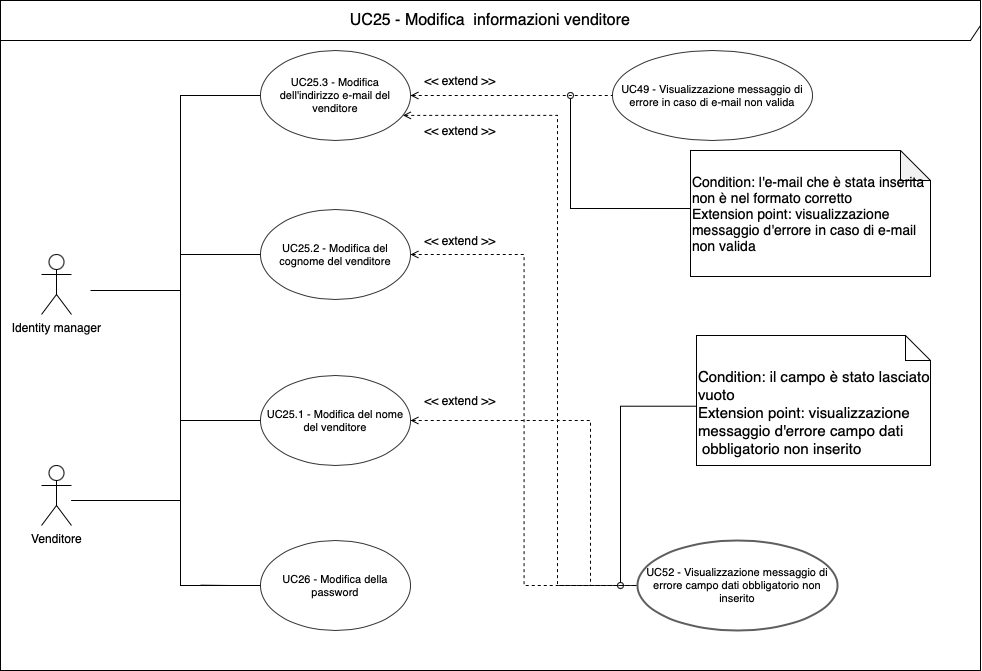
\includegraphics[scale=0.4]{Immagini/DiagrammiUC/Venditore/ModificaInformazioniVenditore.png}
    \caption{Diagramma di \actualUC: Modifica informazioni venditore}
    \label{fig:modifica-informazioni-venditore}
\end{figure}

Il venditore può modificare le sue informazioni personali.
\begin{itemize}
    \item \textbf{Attori primari:} venditore;
    \item \textbf{Attori secondari:} identity manager;
    \item \textbf{Precondizione:} il venditore si trova nella schermata della propria area personale e ha selezionato l'azione di modifica delle proprie informazioni;
    \item \textbf{Postcondizione:} il venditore ha aggiornato le proprie informazioni personali;
    \item \textbf{Scenario principale:} il venditore si trova nella schermata della propria area personale e può compiere le seguenti azioni:
    \begin{itemize}
    	\item (UC\ref{modifica-informazioni-venditore.nome}) - Modifica del nome del venditore;
    	\item (UC\ref{modifica-informazioni-venditore.cognome}) - Modifica del cognome del venditore;
        \item (UC\ref{modifica-informazioni-venditore.email}) - Modifica dell'indirizzo e-mail del venditore;
        \item (UC\ref{modifica-informazioni-venditore.password}) - Modifica della password del venditore;
        \item (UC\ref{modifica-informazioni-venditore.logo}) - Modifica del logo;
        \item (UC\ref{modifica-informazioni-venditore.nome-azienda}) - Modifica nome dell'azienda;
        \item (UC\ref{modifica-informazioni-venditore.descrizione-azienda}) - Modifica della descrizione dell'azienda.
    \end{itemize}
    Il venditore conferma le modifiche compiute e le informazioni personali verranno modificate;
    \item \textbf{Scenari alternativi:}
    \begin{enumerate}[label=\lett]
    	\item Il venditore non conferma le modifiche effettuate e di conseguenza non verranno aggiornate le informazioni personali;
    \end{enumerate}
    \item \textbf{Estensioni:}
    \begin{enumerate}[label=\lett]
    	\item Il venditore compila i campi dati per la password e la conferma della stessa con due password diverse, in questo caso:
    	\begin{itemize}
    		\item L'identity manager segnala che le due password inserite non coincidono;
    		\item (UC\ref{estensione:password-conferma-diverse}) - Visualizzazione messaggio di errore in caso di password e password di conferma diverse;
    		\item Il venditore può modificare le password inserite.
    	\end{itemize}
    	\item Il venditore cambia il proprio indirizzo e-mail con un'e-mail già presente nella piattaforma e l'identity manager lo segnala. In questo caso:
    	\begin{itemize}
    		\item (UC\ref{estensione:cambio-con-email-esistente}) - Visualizzazione messaggio di errore in caso di cambio e-mail con una già utilizzata nella piattaforma;
    		\item Viene fornita al venditore la possibilità di modificare il proprio indirizzo e-mail inserito.
    	\end{itemize}
    \end{enumerate}
\end{itemize}

\subUC{Modifica del nome del venditore}
\label{modifica-informazioni-venditore.nome}

Il venditore vuole modificare il proprio nome.
\begin{itemize}
	\item \textbf{Attori primari:} venditore;
	\item \textbf{Attori secondari:} identity manager;
	\item \textbf{Precondizione:} il venditore si trova nella schermata di modifica delle proprie informazioni;
	\item \textbf{Postcondizione:} il venditore ha aggiornato il proprio nome;
	\item \textbf{Scenario principale:} il venditore modifica il proprio nome;
	\item \textbf{Scenari alternativi:}
	\begin{enumerate}[label=\lett]
		\item Il venditore non modifica l'attuale nome utilizzato e di conseguenza non cambierà.
	\end{enumerate}
	\item \textbf{Estensioni:}
	\begin{enumerate}[label=\lett]
		\item Il venditore non inserisce il nome e l'identity manager controlla il campo dati che risulta essere vuoto, in questo caso:
		\begin{itemize}
			\item (UC\ref{estensione:campo-obbligatorio-non-inserito}) - Viene mostrato un messaggio d'errore campo dati obbligatorio non inserito;
			\item Viene fornita al venditore la possibilità di inserire un nome.
		\end{itemize}
	\end{enumerate} 
\end{itemize}

\subUC{Modifica del cognome del venditore}
\label{modifica-informazioni-venditore.cognome}

Il venditore vuole modificare il proprio cognome.
\begin{itemize}
	\item \textbf{Attori primari:} venditore;
	\item \textbf{Attori secondari:} identity manager;
	\item \textbf{Precondizione:} il venditore si trova nella schermata di modifica delle proprie informazioni;
	\item \textbf{Postcondizione:} il venditore ha aggiornato il proprio cognome;
	\item \textbf{Scenario principale:} il venditore modifica il proprio cognome;
	\item \textbf{Scenari alternativi:}
	\begin{enumerate}[label=\lett]
		\item Il venditore non modifica l'attuale cognome utilizzato e di conseguenza non cambierà.
	\end{enumerate}
	\item \textbf{Estensioni:}
	\begin{enumerate}[label=\lett]
		\item Il venditore non inserisce il cognome e l'identity manager controlla il campo dati che risulta essere vuoto, in questo caso:
		\begin{itemize}
			\item (UC\ref{estensione:campo-obbligatorio-non-inserito}) - Viene mostrato un messaggio d'errore campo dati obbligatorio non inserito;
			\item Viene fornita al venditore la possibilità di inserire un cognome.
		\end{itemize}
	\end{enumerate} 
\end{itemize}

\subUC{Modifica dell'indirizzo e-mail del venditore}
\label{modifica-informazioni-venditore.email}

Il venditore vuole modificare la propria e-mail.
\begin{itemize}
    \item \textbf{Attori primari:} venditore;
    \item \textbf{Attori secondari:} identity manager;
    \item \textbf{Precondizione:} il venditore si trova nella schermata di modifica delle proprie informazioni;
    \item \textbf{Postcondizione:} il venditore ha aggiornato il suo indirizzo e-mail;
    \item \textbf{Scenario principale:} il venditore modifica il proprio indirizzo e-mail;
    \item \textbf{Scenari alternativi:}
    \begin{enumerate}[label=\lett]
    	\item Il venditore non modifica l'attuale indirizzo e-mail utilizzato e di conseguenza non cambierà.
    \end{enumerate}
    \item \textbf{Estensioni:}
    \begin{enumerate}[label=\lett]
    	\item Il venditore ha inserito un indirizzo e-mail e l'identity manager segnala che non è nel formato non corretto, in questo caso:
    	\begin{itemize}
    		\item (UC\ref{estensione:email-non-valida}) - Viene mostrato un messaggio d'errore indirizzo e-mail non rispetta il formato;
    		\item Viene fornita al venditore la possibilità di modificare l'indirizzo e-mail inserito.
    	\end{itemize}
	    \item Il venditore non inserisce l'e-mail e l'identity manager controlla il campo dati che risulta essere vuoto, in questo caso:
	    \begin{itemize}
	    	\item (UC\ref{estensione:campo-obbligatorio-non-inserito}) - Viene mostrato un messaggio d'errore campo dati obbligatorio non inserito;
	    	\item Viene fornita al venditore la possibilità di inserire un indirizzo e-mail.
	    \end{itemize}
    \end{enumerate} 
\end{itemize}

\subUC{Modifica della password del venditore}
\label{modifica-informazioni-venditore.password}

\begin{figure}[H]
    \centering
    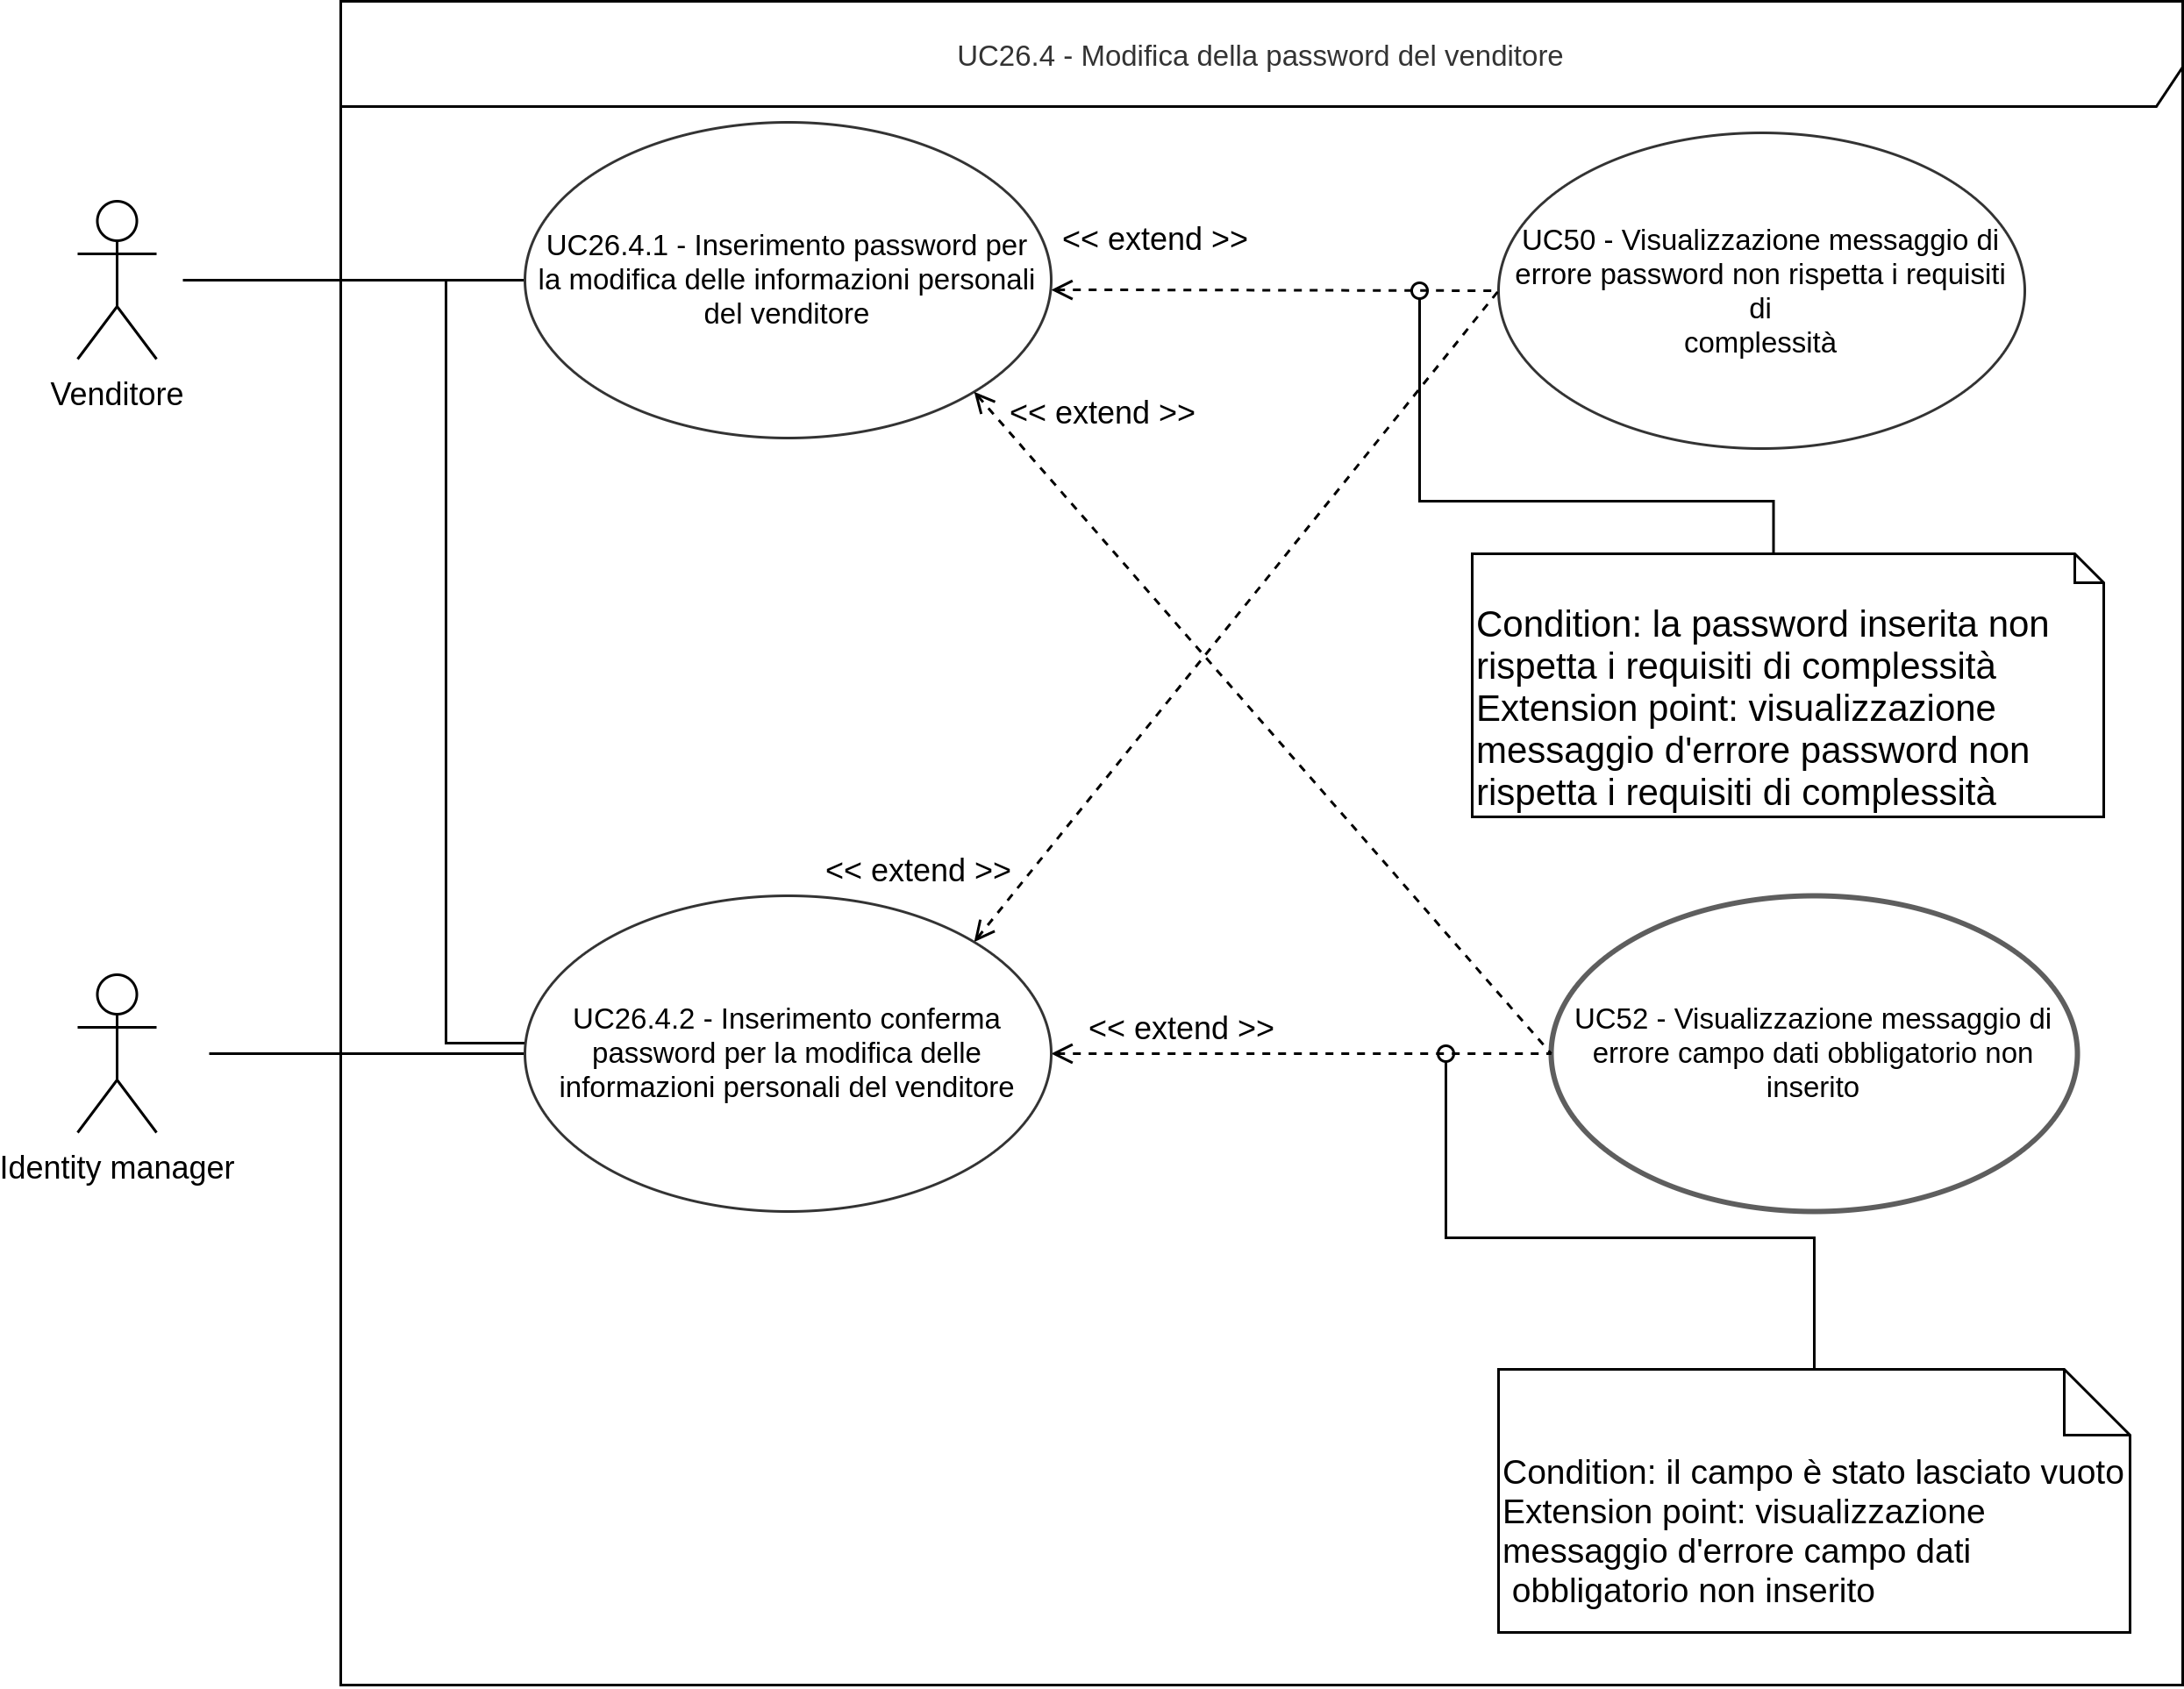
\includegraphics[scale=0.6]{Immagini/DiagrammiUC/Venditore/ModificaPasswordVenditore.png}
    \caption{Diagramma di \actualSubUC: Modifica della password del venditore}
    \label{fig:modifica-informazioni-venditore.password}
\end{figure}

Il venditore vuole modificare la propria password.
\begin{itemize}
    \item \textbf{Attori primari:} venditore;
	\item \textbf{Attori secondari:} identity manager;
    \item \textbf{Precondizione:} il venditore si trova nella schermata di modifica delle proprie informazioni;
    \item \textbf{Postcondizione:} il venditore ha modificato la sua password;
    \item \textbf{Scenario principale:} Il venditore per poter cambiare la password deve compiere i seguenti passi:
        \begin{itemize}
            \item (UC\ref{modifica-informazioni-venditore.password.nuova-password}) - Inserimento password per la modifica delle informazioni personali del venditore;
            \item (UC\ref{modifica-informazioni-venditore.password.conferma-nuova-password}) - Inserimento conferma password per la modifica delle informazioni personali del venditore.
        \end{itemize}
    \item \textbf{Scenari alternativi:}
    \begin{enumerate}[label=\lett]
    	\item Il venditore non modifica la password attuale e per questo non cambierà.
    \end{enumerate}
\end{itemize}

\subSubUC{Inserimento password per la modifica delle informazioni personali del venditore}
\label{modifica-informazioni-venditore.password.nuova-password}

Il venditore inserisce una nuova password.
\begin{itemize}
	\item \textbf{Attori primari:} venditore;
	\item \textbf{Attori secondari:} identity manager;
	\item \textbf{Precondizione:} il venditore non ha ancora fornito una password che rispetta i requisiti di complessità ed ha a disposizione un campo dati dove inserirla;
	\item \textbf{Postcondizione:} il venditore ha inserito una password valida;
	\item \textbf{Scenario principale:} il venditore inserisce una password che rispetta le condizioni imposte;
	\item \textbf{Estensioni:}
	\begin{enumerate}[label=\lett]
		\item Il venditore elimina la propria password attuale, non ne inserisce una nuova e l'identity manager lo segnala. In questo caso:
		\begin{itemize}
			\item (UC\ref{estensione:campo-obbligatorio-non-inserito}) - Viene mostrato un messaggio d'errore campo dati obbligatorio non inserito;
			\item Viene fornita all'utente la possibilità di inserire una password.
		\end{itemize}
		\item Il venditore ha inserito una password che non rispetta i requisiti minimi di complessità e l'identity manager lo segnala. In questo caso:
		\begin{itemize}
			\item (UC\ref{estensione:password-non-valida}) - Viene mostrato un messaggio d'errore password non rispetta i requisiti di complessità;
			\item Viene fornita al venditore la possibilità di modificare la password inserita.
		\end{itemize}
	\end{enumerate} 
\end{itemize}

\subSubUC{Inserimento conferma password per la modifica delle informazioni personali del venditore}
\label{modifica-informazioni-venditore.password.conferma-nuova-password}

Il venditore inserisce la conferma della nuova password.
\begin{itemize}
	\item \textbf{Attori primari:} venditore;
	\item \textbf{Attori secondari:} identity manager;
	\item \textbf{Precondizione:} il venditore non ha ancora fornito una password che rispetta i requisiti di complessità ed ha a disposizione un campo dati dove inserirla;
	\item \textbf{Postcondizione:} il venditore ha inserito la conferma della password ed è valida;
	\item \textbf{Scenario principale:} il venditore inserisce una password che rispetta le condizioni imposte;
	\item \textbf{Estensioni:}
	\begin{enumerate}[label=\lett]
		\item Il venditore elimina la conferma della propria password attuale, non ne inserisce una nuova e l'identity manager lo segnala. In questo caso:
		\begin{itemize}
			\item (UC\ref{estensione:campo-obbligatorio-non-inserito}) - Viene mostrato un messaggio d'errore campo dati obbligatorio non inserito;
			\item Viene fornita all'utente la possibilità di inserire una password.
		\end{itemize}
		\item Il venditore ha inserito una password, come conferma della password, che non rispetta i requisiti minimi di complessità e l'identity manager lo segnala. In questo caso:
		\begin{itemize}
			\item (UC\ref{estensione:password-non-valida}) - Viene mostrato un messaggio d'errore password non rispetta i requisiti di complessità;
			\item Viene fornita al venditore la possibilità di modificare la password inserita.
		\end{itemize}
	\end{enumerate} 
\end{itemize}

\subUC{Modifica del logo}
\label{modifica-informazioni-venditore.logo}

Il venditore vuole modificare il proprio logo.
\begin{itemize}
    \item \textbf{Attori primari:} venditore;
    \item \textbf{Precondizione:} il venditore si trova nella schermata di modifica delle proprie informazioni;
    \item \textbf{Postcondizione:} il venditore ha inserito un nuovo logo aziendale;
    \item \textbf{Scenario principale:} il venditore modifica il proprio logo aziendale scegliendo un'immagine tra quelle disponibili localmente nel proprio dispositivo;
    \item \textbf{Scenari alternativi:}
    \begin{enumerate}[label=\lett]
    	\item Il venditore non seleziona alcun file ed il logo non verrà cambiato.
    \end{enumerate}
    \item \textbf{Estensioni:}
    \begin{enumerate}[label=\lett]
    	\item Il venditore seleziona un file del tipo non immagine. In questo caso:
    	\begin{itemize}
    		\item (UC\ref{estensione:file-no-tipo-immagine}) - Verrà visualizzato il messaggio di errore il quale segnala che il file selezionato non è del tipo immagine;
    		\item Viene fornita al venditore la possibilità di modificare il file inserito.
    	\end{itemize}
    \end{enumerate}
\end{itemize}

\subUC{Modifica nome dell'azienda}
\label{modifica-informazioni-venditore.nome-azienda}

Il venditore vuole modificare il nome dell'azienda.
\begin{itemize}
	\item \textbf{Attori primari:} venditore;
	\item \textbf{Precondizione:} il venditore si trova nella schermata di modifica delle proprie informazioni;
	\item \textbf{Postcondizione:} il venditore ha aggiornato il nome dell'azienda;
	\item \textbf{Scenario principale:} il venditore modifica il nome della propria azienda;
	\item \textbf{Scenari alternativi:}
	\begin{enumerate}[label=\lett]
		\item Il venditore non modifica l'attuale nome aziendale utilizzato e di conseguenza non cambierà.
	\end{enumerate}
	\item \textbf{Estensioni:}
	\begin{enumerate}[label=\lett]
		\item Il venditore non inserisce il nome aziendale ed il campo dati risulta essere vuoto. In questo caso:
		\begin{itemize}
			\item (UC\ref{estensione:campo-obbligatorio-non-inserito}) - Viene mostrato un messaggio d'errore campo dati obbligatorio non inserito;
			\item Viene fornita al venditore la possibilità di inserire un nome aziendale.
		\end{itemize}
	\end{enumerate} 
\end{itemize}

\subUC{Modifica della descrizione dell'azienda}
\label{modifica-informazioni-venditore.descrizione-azienda}

Il venditore vuole modificare la descrizione dell'azienda che viene mostrata nella schermata principale.
\begin{itemize}
    \item \textbf{Attori primari:} venditore;
    \item \textbf{Precondizione:} il venditore si trova nella schermata di modifica delle proprie informazioni;
    \item \textbf{Postcondizione:} il venditore ha aggiornato la descrizione dell'azienda;
    \item \textbf{Scenario principale:} il venditore modifica la descrizione dell'azienda;
    \item \textbf{Scenari alternativi:}
    \begin{enumerate}[label=\lett]
    	\item Il venditore non modifica l'attuale descrizione dell'azienda e di conseguenza non cambierà.
    \end{enumerate}
\end{itemize}